\documentclass[20 pts]{article}
\usepackage{xeCJK}
\usepackage{amsfonts}
\usepackage{amssymb}
\usepackage{amsmath}
\usepackage{bm}
\setCJKmainfont{SimSun}
\title{Simulation of Turbo Codes}
\author{Kwame Ackah Bohulu}
\date{27-04-2017}
\begin{document}
\maketitle


\section{Introduction}


\section{Block Interleavers and Linear Interleavers}
A block interleaver is a deterministic interleaver definded by a rectangular matrix of size $N=m\times n$. The input bits are written row-wise and read column-wise. The index mapping function of a block interleaver is defined in (1) below[00868474]

$$\Pi_{\mathfrak{B}_N} \equiv ni + \lfloor1/m\rfloor \mod {N},		0\leq i < N.$$
The index mapping function of a linear interleaver is defined by (2) below

$$\Pi_{\mathfrak{L}_N} \equiv ki + v \mod {N},		0\leq i < N.$$
where $k$ is a fixed integer which is relatively prime to N and v is a fixed integer.

It is noted that the linear interleaver ''linearizes'' the $\lfloor ・\rfloor$ portion of (1). 
Block and Linear interleavers are both based on linear congruence and therefore essentially have the same properties. For example in block interleavers,two elements seperated by a constant $t\mod {N}$ in an input sequence  almost always map to an output sequence with corresponding elements seperated by a fixed constant $tn\mod{n}$ whiles for linear interleavers, they always map to output sequences with corresponding elements separated by a fixed constant $tk\mod{N}$. The constant $k$ is called the angular coefficient of the linear interleaver[00868474] and for the block interleaver this is equal to the interleaver depth. Due to the similarity in properties the analysis of the block interleaver can be done using the linear interleaver model.

The performance of the interleaver is affected by its angular coefficient (interleaver depth) as is established in [11]. When used in Turbo codes, linear interleavers are prone to ''bad'' input sequences of weight 2 and weight 4, especially those of input weight 2. A ''bad input sequence'' is one that outputs  a low weight codeword in Turbo codes. In the case of ''bad'' weight 4 input sequences, changing the angular coefficient has no effect on improving the performance of the turbo code. However, In the case of ''bad'' weight 2 input sequences, changing the angular coefficient using the specified technique below helps to avoid such bad input sequences.

To guarantee the minimum value of the sum of the distances between the projection of two lattice points on the x-axis and the distance between the projection of the same points on the y-axis is approximately $\sqrt{2N}$, angular coefficient of $\sqrt{2N}$ or integer value close to it is required.[12]  It is however shown that angular coefficient value of $\sqrt{N} $ is also a good choice meaning there is a large minimum distance between the points in the lattice which ensures a large minimum distance for the weight 2 input sequences of Turbo codes when this interleaver is used.



A graph of two linear interleavers are shown in Figs. 1 and 2 below
\begin{figure}[h!]
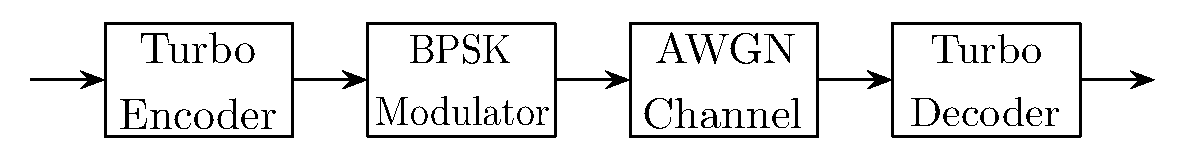
\includegraphics[width=10cm]{figure4.pdf}
\caption{システムモデル}
\label{}
\end{figure}
\subsection{ターボ符号器}
ターボ符号器、二つの畳み込み符号(要素符号器)をインタリーバで並列連結することで作られている。入力はバイナリの情報系列であり、出力はターボ復号である。ターボ符号器の図は、図2に書かれている。
\begin{figure}[h!]
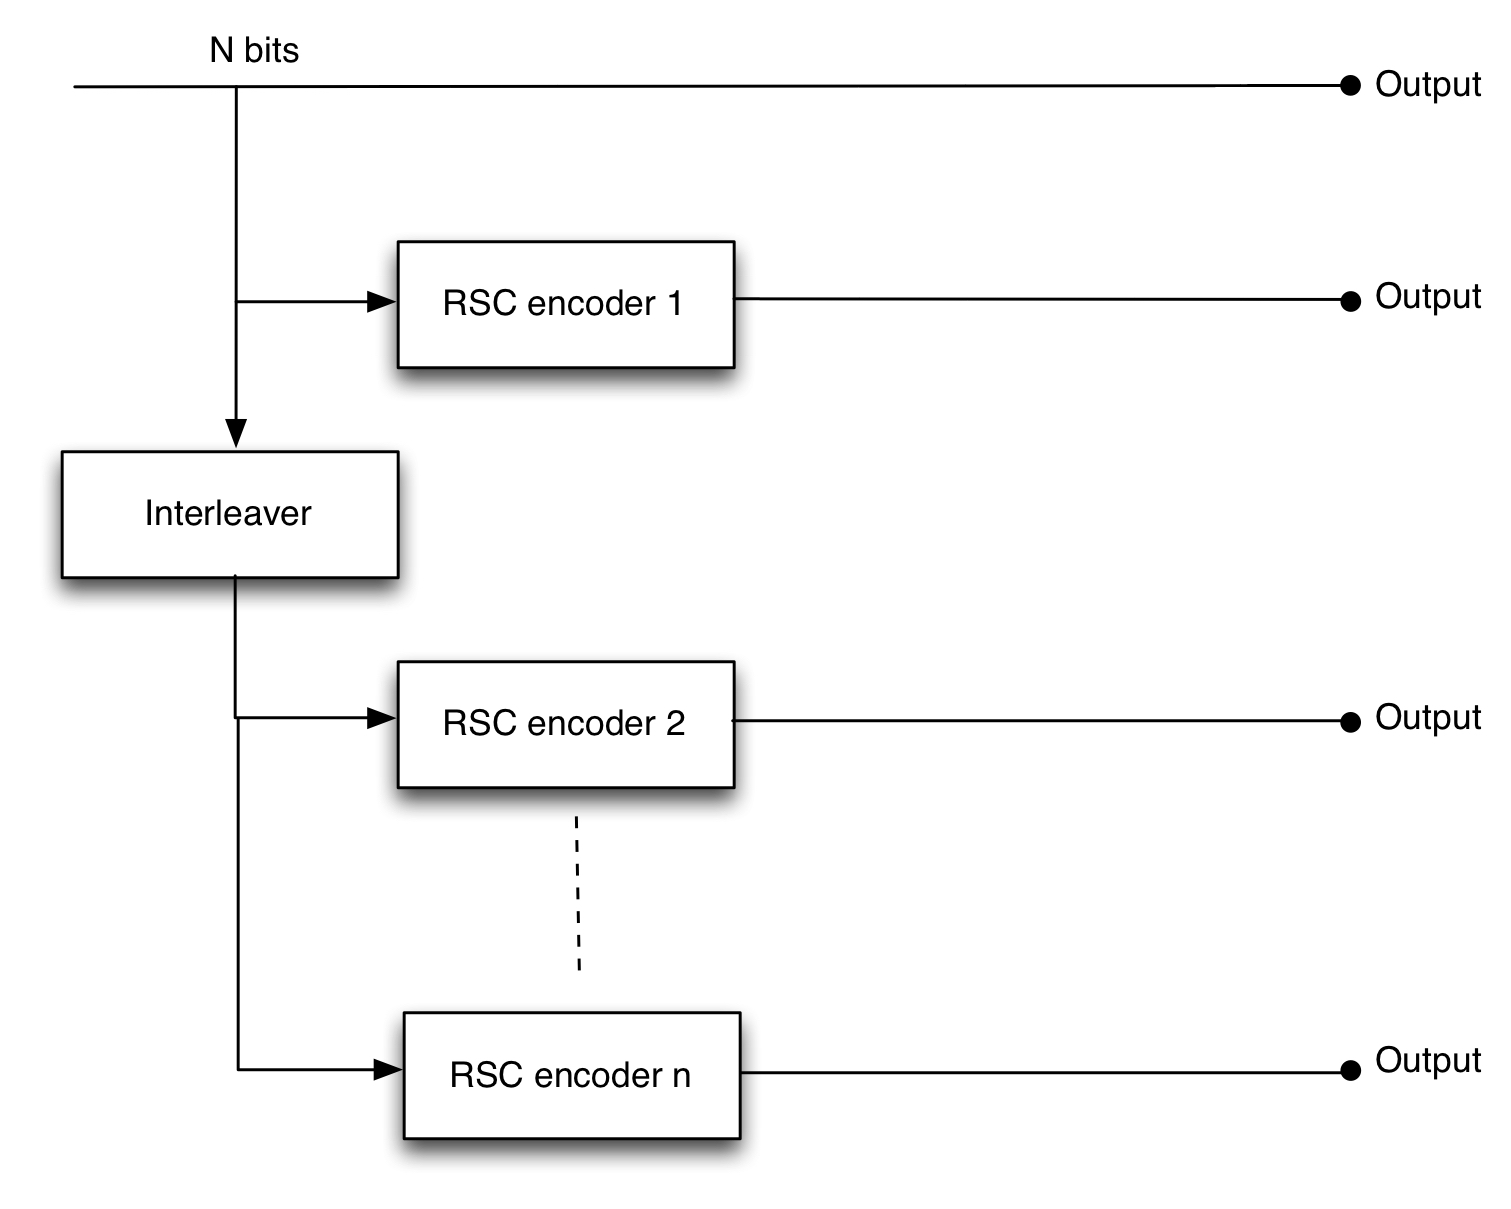
\includegraphics[width=10cm]{turboencoder.jpg}
\caption{ターボ符号器}
\label{}
\end{figure}
要素符号器は、同じで、5/7, k=1,n=2,K=3 RSC符号器である。利用したインタリーバは置換多項式に基づいてインタリーバ[5]とブロックインタリーバである。インタリーバの長さは、情報系列の長さと同じである。パンクチュアリングはしないので、ターボ符号器のレートは1/3である。ターボ符号器のプログラムは図3に書かれている。
\begin{figure}[h!]
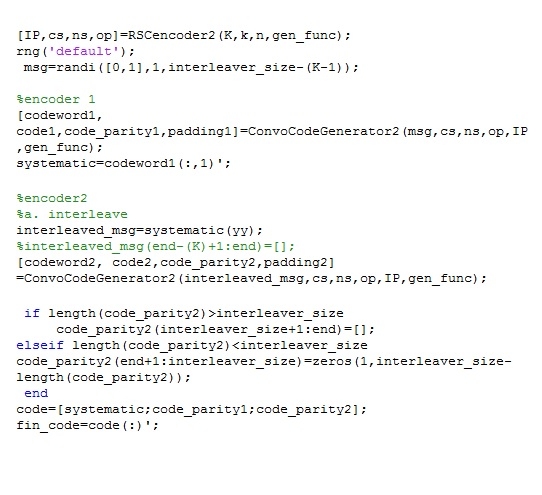
\includegraphics[width=10cm]{zu3.jpg}
\caption{ターボ符号器プログラム}
\label{}
\end{figure}
\subsection{BPSK変調器とAWGNチャネル}
ターボ復号器の出力は、BPSK変調器の入力になる。入力ビットが$0$の場合、出力が$-1$になり、入力ビットが$1$の場合、出力が$-1$になる。BPSK変調器の出力は、AWGNチャネルで送信する。BPSK変調器とAWGNチャネルのプログラムは図4書かれている。
\begin{figure}[h!]
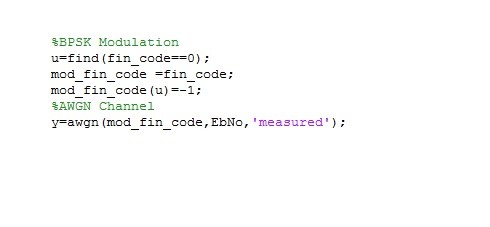
\includegraphics[width=10cm]{zu4.jpg}
\caption{BPSK変調器とAWGNチャネルプログラム}
\label{}
\end{figure}

\subsection{ターボ復号器}
ターボ復号器の図は図5に書かれている。SISOの復号器が利用されるので、BPSK復調はしない。ターボ復号器の入力は、AWGNチャネルの出力であり、系統的ビットと二つのパリティービットに分別する。1番目のSISO復号器の入力は系統的ビットと1番目のパリティービットであり、2番目のSISO復号器は、インタリーバで並び替えされた系統的ビットと2番目のパリティービットである。	
\begin{figure}[h!]
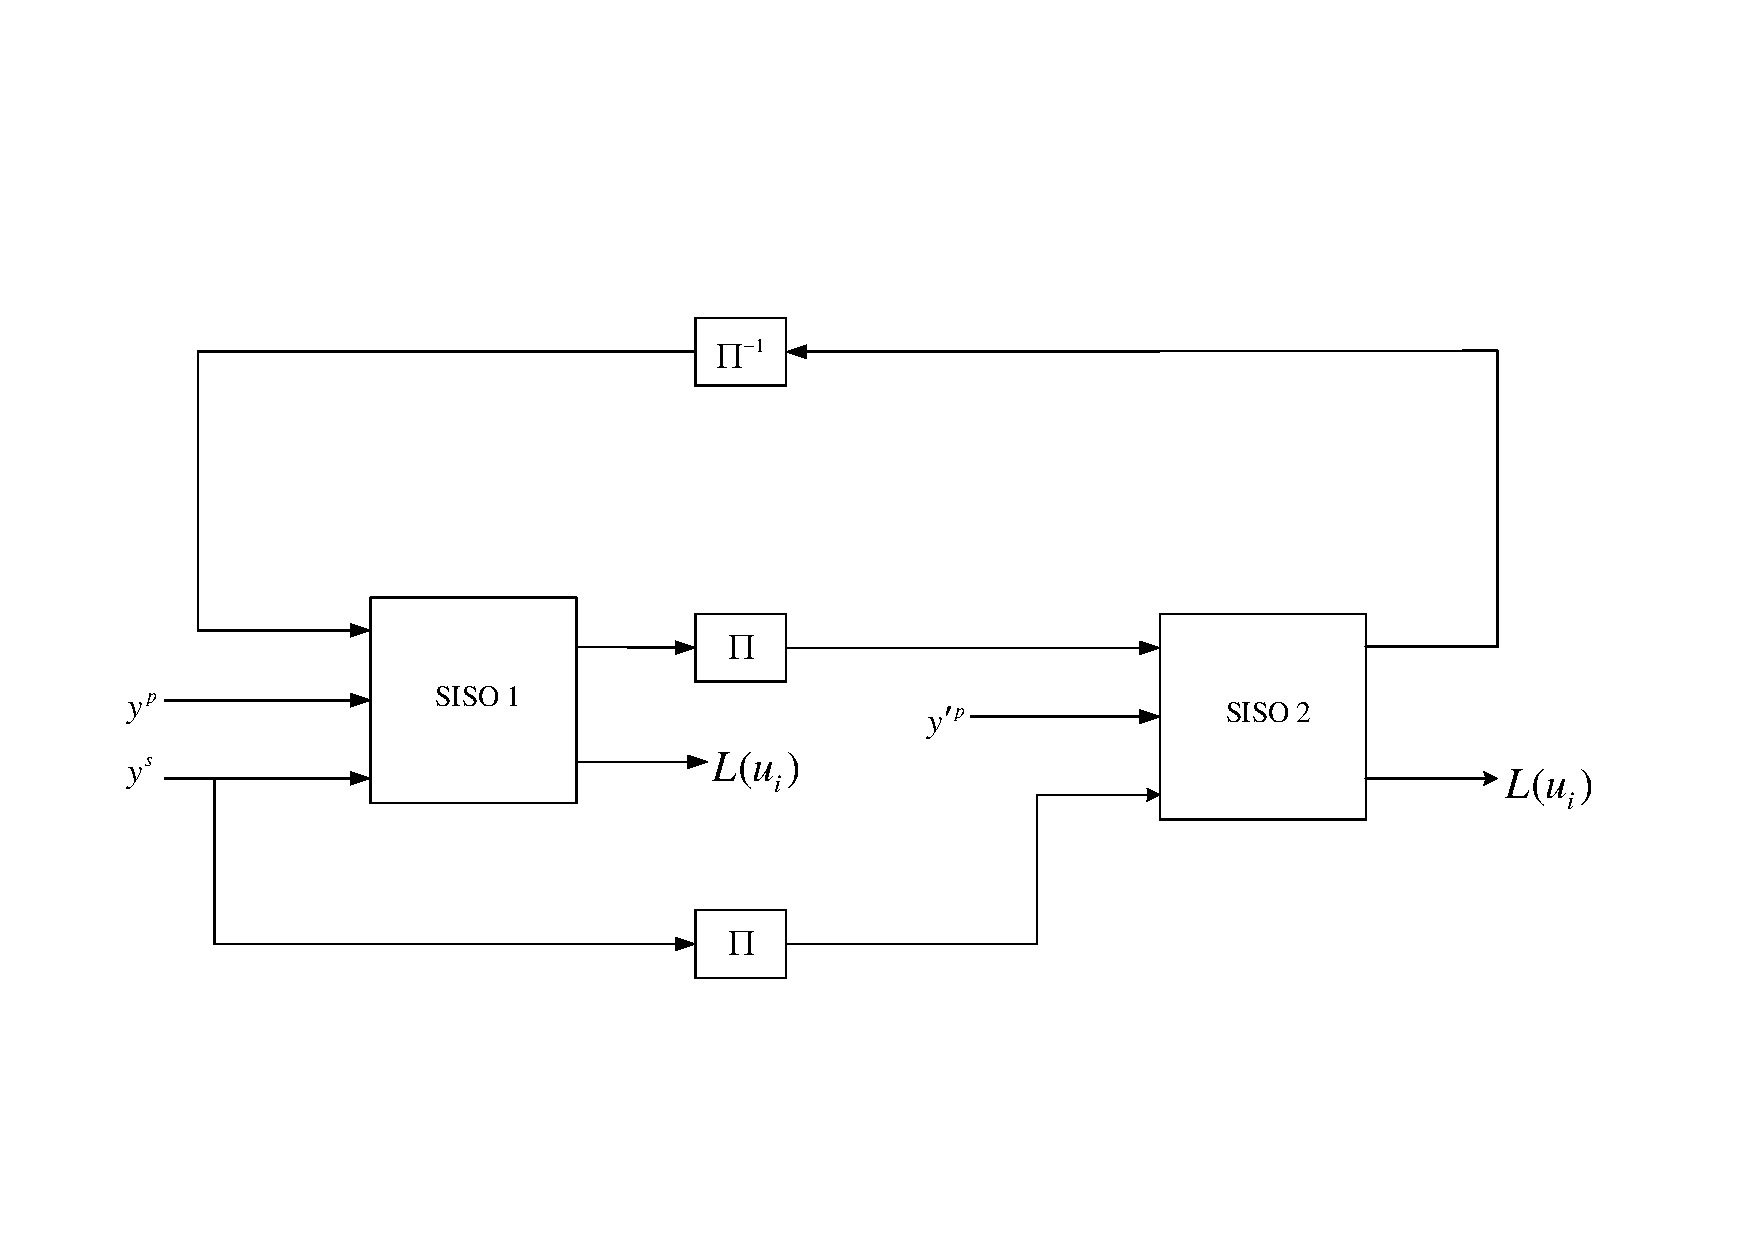
\includegraphics[width=10cm]{D1.pdf}
\caption{ターボ復号器}
\label{図2}
\end{figure}%
両方のSISO復号器は、Max-Log-MAP アルゴリズムを再帰的に利用して復号する。ターボ復号器の出力は、入力のLLR値であり、最後の反復になったら、それ をデインタリーブして、情報系列 の値を評価する。ターボ復号器のプログラムは図6に書かれている。

\begin{figure}[h!]
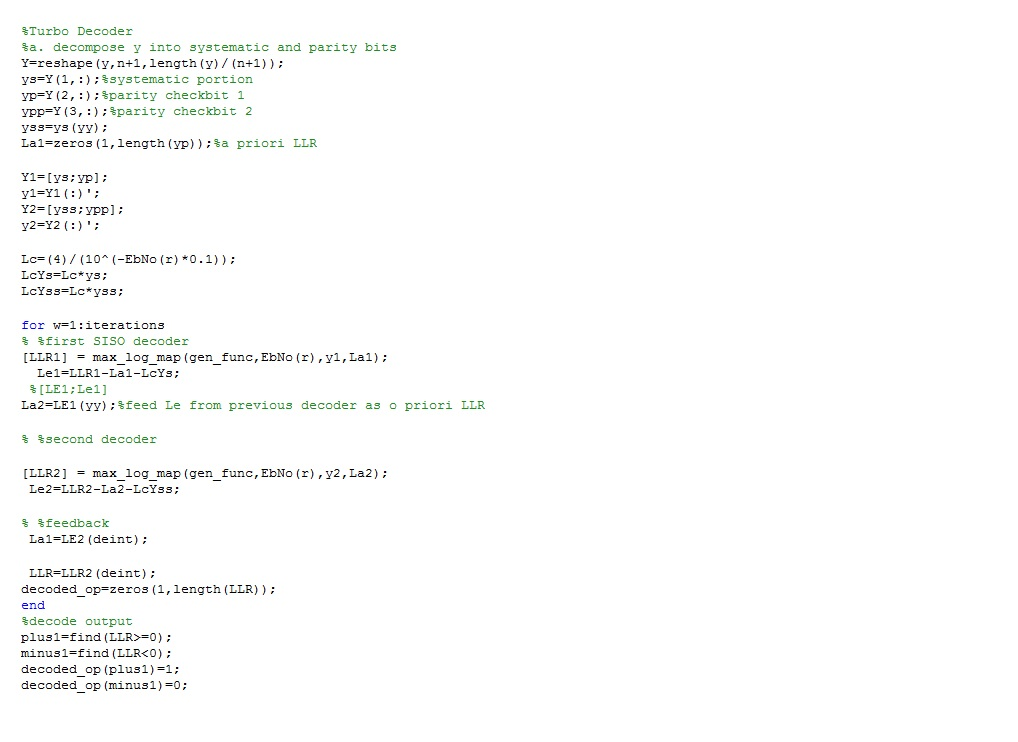
\includegraphics[width=10cm]{zu6.jpg}
\caption{ターボ復号器のプログラム}
\label{図2}
\end{figure}

\section{Max-log-MAPアルゴリズムの実現方法}
Max-log-MAPアルゴリズムは、対数領域のBCJR アルゴリズムである。BPSK変調とAWGNチャネルの場合は、式1-3を使用して復号する。

\begin{equation}\widetilde{\gamma}(s',s)= \ln P(u_i)+(\frac{2y_i^sc_i^s}{N_o})+(\frac{2y_i^pc_i^p}{N_o})\end{equation}
\begin{equation}
\begin{split}
&\widetilde{\alpha}_i(s)=\max_{s'}\{\widetilde{\alpha}_{i-1}(s')+\widetilde{\gamma}(s',s)\}\\
&\widetilde{\beta}_{i-1}(s)=\max_{s}\{\widetilde{\beta}_{i}(s')+\widetilde{\gamma}(s',s)\}
\end{split}
\end{equation}

\begin{equation}
\begin{split}
L(u_i)=&\max_{R_1}\Big\{\widetilde{\alpha}_{i-1}(s')+\widetilde{\gamma}(s',s)+(\widetilde{\beta}_{i}(s')\Big\}-\\&\max_{R_0}\Big\{\widetilde{\alpha}_{i-1}(s')+\widetilde{\gamma}(s',s)+(\widetilde{\beta}_{i}(s')\Big\}
\end{split}
\end{equation}
\begin{equation}L^{(e)}(u_i)=L(u_i)-\Big(L_cy_i^s+L^{(a)}(u_i)\Big)\end{equation}
$L_cy_i^s=\frac{4\sqrt{\varepsilon_c}y_i^s}{N_o}$はチャネルの$L(u_i)$値を示し、組織的なビットの影響に関するチャネルの出力を表れる。\\
$L^{(a)}(u_i)=\ln\frac{P(u_i)=1}{P(u_i)=0}$は先天的な(a priori)$ L(u_i)$値である。\\
$L^{(e)}(u_i)$は、外因性$L(u_i)$の値を示し、パリティビットに関する$L(u_i)$の値である。

両方の場合は、以下の初期条を利用する。
\[
    \widetilde{\alpha}_0(s)= 
\begin{cases}
   0,& s= 0\\        -\infty,              &  s\neq 0
\end{cases}
\]

\[
   \widetilde{\beta}_N(s)= 
\begin{cases}
   0,& s= 0\\        -\infty,              &  s\neq 0
\end{cases}
\]
$\widetilde{\alpha}_i(s)$は、時間がi-1のとき、状態が$s'$で今まで受信された系列は$(\boldsymbol{y}_{<i}$の共同確率を表す。\\
$\widetilde{\gamma}(s',s)$は、過去の状態が$s'$の条件で未来の状態が$s$であり、受信された系列が$\boldsymbol{y}_{i}$である確率を表す。\\
$\widetilde{\beta}_{i-1}(s)$は、現在の状態が$s$の条件で未来の系列は$\boldsymbol{y}_{>i}$になるの条件付確率を表す。

Max-Log-MAPアルゴリズムを実現するため、図7に書かれている 5/7, k=1,n=2,K=3 RSC符号器trellisを使って説明する。
\begin{figure}[h!]
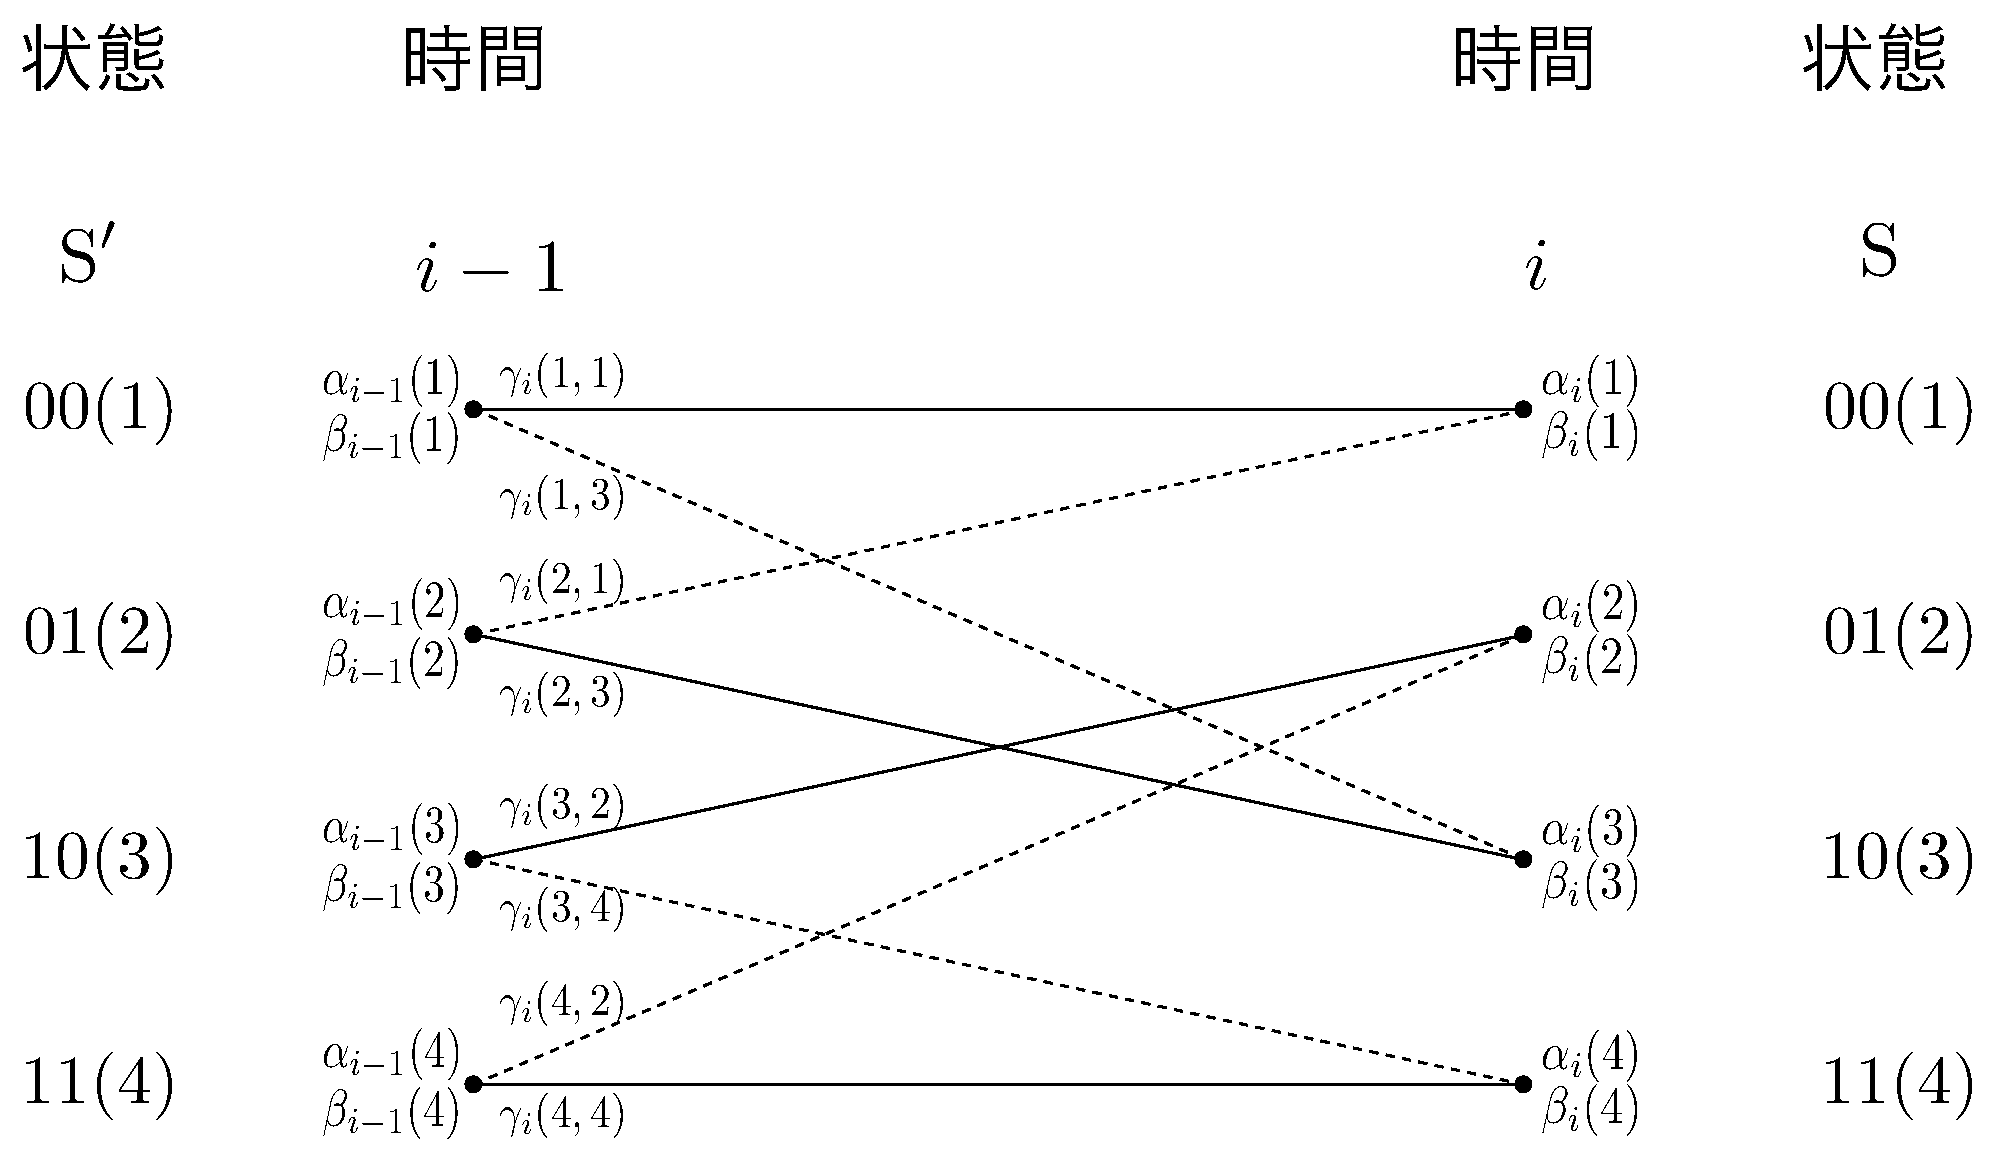
\includegraphics[width=10cm]{figure3.pdf}
\caption{5/7, k=1,n=2,K=3 RSC符号器のtrellis}
\label{図2}
\end{figure}
\subsection{$\widetilde{\gamma}(s',s)$の計算方法}
$\widetilde{\gamma}(s',s)$を計算するために、trellisの状態遷移を保存する必要があります。$\widetilde{\alpha}_i(s)$と$\widetilde{\beta}_{i-1}(s)$の計算にも必要である。$\widetilde{\gamma}(s',s)$のプログラムは図8に書かれている。
\begin{figure}[h!]
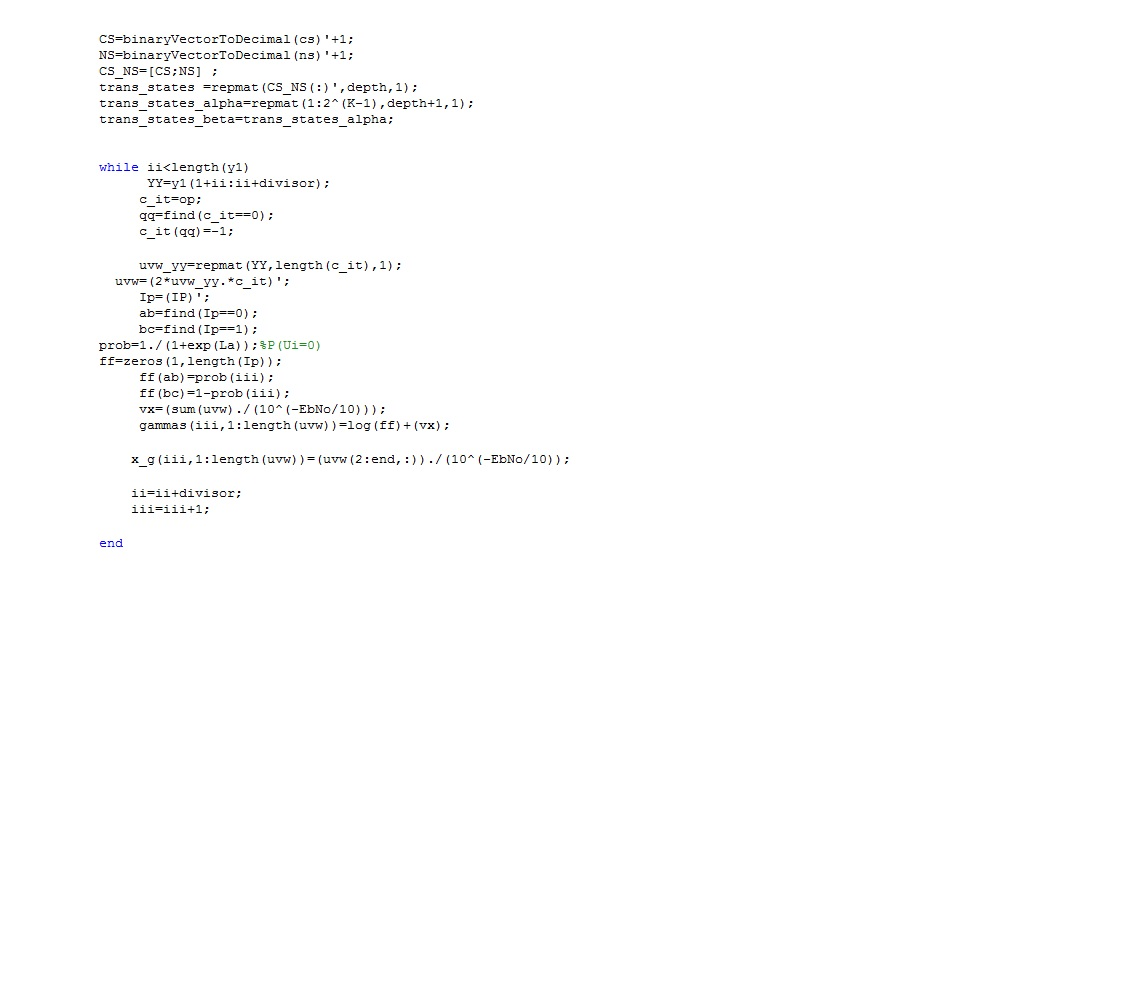
\includegraphics[width=10cm]{zu8.jpg}
\caption{$\widetilde{\gamma}(s',s)$のプログラム}
\label{図2}
\end{figure}


\subsection{ $\widetilde{\alpha}_i(s)$と$\widetilde{\beta}_{i-1}(s)$の計算方法}
式2で$\widetilde{\alpha}_i(s)$と$\widetilde{\beta}_{i-1}(s)$の計算ができる。計算するのに、$\widetilde{\gamma}(s',s)$の値が必要である。例えば、保存されたtrellisの状態遷移は表1に書かれている。
\begin{center}
\begin{tabular}{ |c|c| } 
 \hline
 左 & 右 \\ 
 \hline
 1 & 1 \\ 
 1 & 3  \\ 
 2 & 3  \\ 
 2 & 1 \\ 
 3 & 4  \\ 
 3 & 2  \\ 
 4 & 2 \\ 
 4 & 4  \\ 
 \hline
\end{tabular}
\end{center}
 $\widetilde{\alpha}_i(s)$を計算する場合、右側の値は、次の$\widetilde{\alpha}_i(s)$を計算すのに、どちらの$\widetilde{\gamma}(s',s)$を使用すればいいのかを示す。左側の値は、どちらの前の$\widetilde{\alpha}_i(s)$の値を使用すればいいのかを示す。

$\widetilde{\beta}_{i-1}(s)$を計算する場合、左側の値は、次の$\widetilde{\beta}_{i-1}(s)$を計算すのに、どちらの$\widetilde{\gamma}(s',s)$を使用すればいいのかを示す。右側の値は、どちらの前の$\widetilde{\beta}_{i-1}(s)$の値を使用すればいいのかを示す。図9の考え方で、$\widetilde{\alpha}_i(s)$と$\widetilde{\beta}_{i-1}(s)$の計算が簡単にできる。

\begin{figure}[h!]
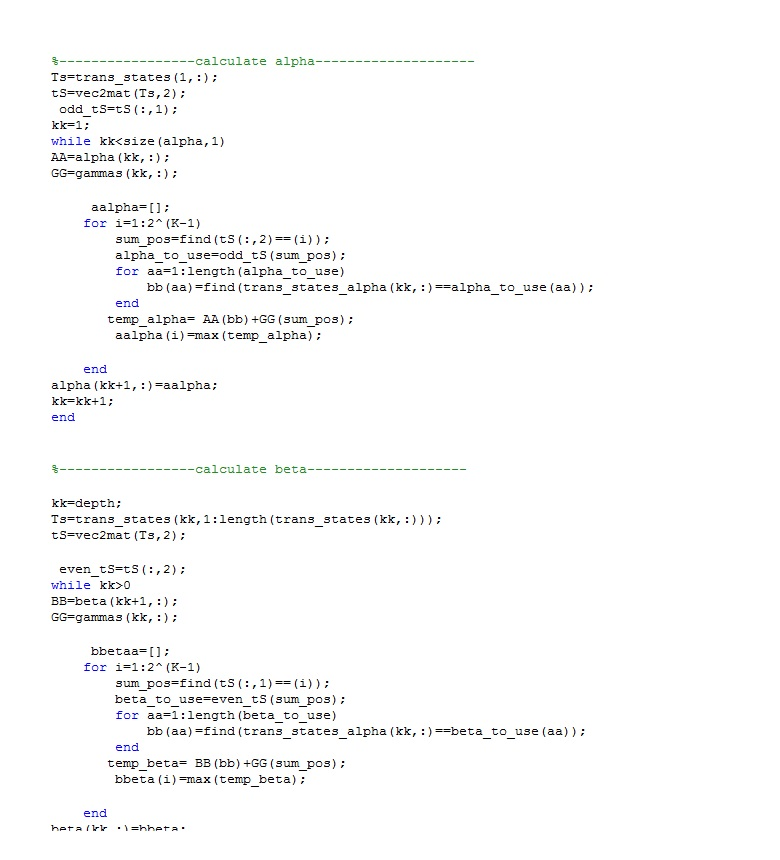
\includegraphics[width=10cm]{zu9.jpg}
\caption{ $\widetilde{\alpha}_i(s)$と$\widetilde{\beta}_{i-1}(s)$のプログラム}
\label{図2}
\end{figure}

\subsection{$L^{(e)}(u_i)$と$L(u_i)$の計算方法}
$L(u_i)$は、式3で計算される。最初に時間がiのときの$\widetilde{\gamma}(s',s)$の値は、情報ビット0に関する値(分母)と情報ビット1に関する値(分子)に分ける。次にそれぞれの$\widetilde{\gamma}(s',s)$どちらの$\widetilde{\alpha}_i(s)$と$\widetilde{\beta}_{i-1}(s)$と足し算すればいいのかを決める。次に、分子の和から分母の和を引く。最後に、式4を使って、$L^{(e)}(u_i)$を計算する。
$L^{(e)}(u_i)$と$L(u_i)$のプログラムは図10に書かれている。
注意:2番目のSISO復号器の$L^{(a)}(u_i)$はインタリーブされた$L^{(e)}(u_i)$になるので、それを使って、$\widetilde{\gamma}(s',s)$、$\widetilde{\alpha}_i(s)$と$\widetilde{\beta}_{i-1}(s)$をまた計算しなくてはいけない。
\begin{figure}[h!]
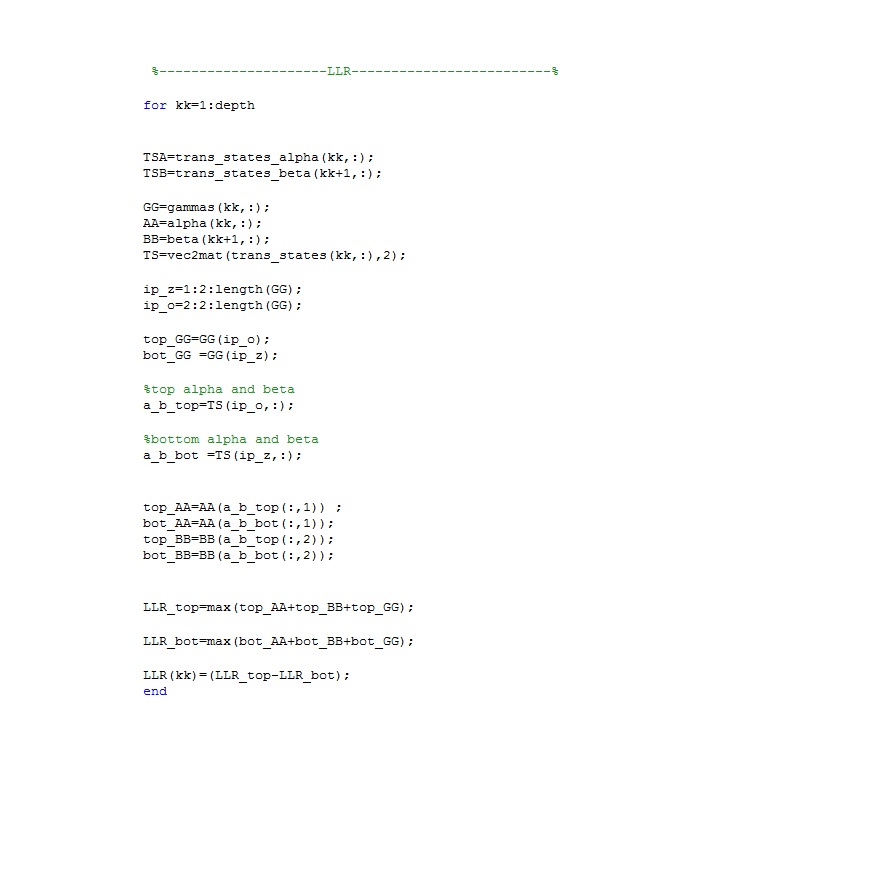
\includegraphics[width=10cm]{zu10.jpg}
\caption{ $L(u_i)$ののプログラム}
\label{図2}
\end{figure}

\newpage
\section{References}
\paragraph{[1]}   John G. Proakis, Masoud Salehi. ''Digital Communications'', Fifth Edition,Chapter 8, McGraw-Hill\\.
\paragraph{[2]}  Oscar Y. Takeshita, Member, IEEE, and Daniel J. Costello ,''New Deterministic Interleaver Designs for Turbo Codes'',IEEE Trans. Inform. Theory, vol.  46,pp. 1988-2006,Nov. 2000\\
\paragraph{[3]}  L. C. Perez, J. Seghers, D. J. Costello, Jr., ''A distance spectrum interpretation of turbo codes'', IEEE Trans. Inform. Theory, vol. 42, pp. 1698-1709, Nov. 1996.\\
\paragraph{[4]}  C. Berrou, A. Glavieux and P. Thitimajshima, ''Near Shannon limit error-correcting coding and
decoding: Turbo codes'', Proc. Intern. Conf. Communications (ICC), Geneva, Switzerland, pp. 1064-
1070, May 1993. \\
\paragraph{[5]}  Jing Sun, Oscar Y. Takeshita ''Interleavers for Turbo Codes Using Permutation Polynomials over Integer Rings'', IEEE Trans. Inform. Theory, vol. 51, pp. 101 - 119  Jan. 2005\\


\end{document}